\section{From the arguments to actual \texttt{Prf PRAAx} endpoints}\label{sec:formalization}

The formalization target is a derivation in the object theory, not just a
Lean proof about ordinary natural numbers, rational functions, or metric spaces.
This section specifies the bridge and the remaining work sufficiently precisely
that the mathematical claims can be implemented module by module. The supplied
Lean files record definitions and proof obligations; they are not a completed
formalization of the analytic results.

\subsection{A contract stores its derivation}

The useful minimal interface is a formula together with its residual assumptions
and a proof object:
\begin{quote}\ttfamily\small
structure CompiledContract (n : Nat) where\\
\hspace*{1em}premises : List (Fm PTm n)\\
\hspace*{1em}conclusion : Fm PTm n\\
\hspace*{1em}derivation : Prf PRAAx premises conclusion
\end{quote}
It cannot be constructed merely by attaching an informal claim or a successful
Python calculation. To discharge its premises, supply an actual object
derivation for every formula in the premise list and use \texttt{Prf.trans}.
To specialize numerical parameters, use \texttt{Prf.subst}. Both operations
are present in the inspected \texttt{Deduction.lean}. The archive's
\texttt{ObjectContracts.lean} implements these wrappers against those APIs.

If a derivation assumes ``the evaluator satisfies a Lipschitz law'', that
formula stays in its context until a derivation for the concrete evaluator
has been supplied. If a numerical input carries a finite certificate, a
separate theorem establishes what the certificate check implies. These are
different situations and must not share an ambiguous status such as ``proved
conditional on certification''.

\subsection{The numerical definitions required by the main lemmas}

The base library needs total code functions for rational addition, multiplication,
absolute value, order, powers of two, finite sums and maxima, vector coordinates,
and Gaussian-rational division with a positive-denominator guard. Their defining
equations are \texttt{PR} definitions. Rational inequalities below abbreviate
equivalent integer comparisons after multiplication by their recorded positive
denominators. No real arithmetic is hidden in a checker.

For the metric and model-theory layer, fix the following primitive-recursive
families, with numerical parameters $p$ suppressed:
\[
\begin{gathered}
 \mathsf{Valid}(a),\quad d(a,b),\quad
 t(K),\quad \mathsf{Net}(K,j),\quad \mathsf{Select}(K,a),\\
 \mathsf{Atom}(i,K,\bar a),\quad W_i,\quad C_i,\quad
 \mathsf{WF}(s),\quad \mathsf{EvalFormula}(s,K,\bar a).
\end{gathered}
\]
The net selector has the explicit contract
\[
 \mathsf{Valid}(a)\to
 \bigl(\mathsf{Select}(K,a)<t(K)\ \land\
 d(a,\mathsf{Net}(K,\mathsf{Select}(K,a)))\le2^{-K}\bigr).
\]
The atomic contract is the cross-precision inequality
\eqref{eq:model-atoms}. Formula syntax uses finite tags for atoms, rational
connectives, and infimum/supremum binders; environments are coded lists.
Validity checks ensure that each variable index is in range and that all
quantifier nets are nonempty. Evaluation is a bounded traversal of the
finite environment/syntax table. The binder adds a coordinate, rather than
quantifying over an actual real type in the evaluator.

The main numerical model-theory endpoint is the universal closure of
\eqref{eq:model-comparison}, with the net and atomic contracts as premises.
The induction invariant is a Boolean conjunction of the rational inequalities
for the already evaluated table entries. The sizes of both compared
environment tables are bounded, as described in
Section~\ref{sec:continuous-models}. This is the place to reuse
\texttt{BoundedSyntax}, bounded search, and net-transfer lemmas. An induction
on the external Lean proposition ``every continuous assignment satisfies the
formula'' would miss the object-theory requirement.

For ODEs, define fixed numerical functions
\[
 \mathsf{EulerNode}(p,N,q,j),\quad
 \mathsf{Polygon}(p,N,q,t),\quad N(p,n),\quad q(p,n)
\]
from the rational field evaluator. The dimension, field parameters and all
tube constants are in $p$; the field program syntax is fixed. The first
essential endpoint has the exact shape
\begin{equation}\label{eq:ode-object-target}
\begin{split}
 \ipra\vdash \forall p,n,m,t\quad
 H_F(p)\land 0\le t\le T(p)\ \longrightarrow\\
 \left\|\mathsf{Polygon}(p,N(p,n),q(p,n),t)
       -\mathsf{Polygon}(p,N(p,m),q(p,m),t)\right\|_\infty
       \le2^{-n-3}+2^{-m-3}.
\end{split}
\end{equation}
All variables here are numerical codes, including $t$. The premise $H_F$
expands the two evaluator inequalities and the positive tube bounds. The
output is a rational inequality. The new work is to derive the tube invariant
and the common-refinement recurrence for these \emph{actual} functions, then
instantiate the existing rational Gronwall theorem.

For the integral equation, define its right-hand side as a regular name by
the specified quadrature program. Equality means its cross-precision
distance formula, not Lean's definitional equality of two programs. To
establish a requested equality observation, first compute a sufficiently
fine Euler index, then a sufficiently fine Riemann-sum index, then the
evaluation precisions. The inequalities in
Section~\ref{sec:analytic-realization} give each demand explicitly.

For the complex transform, the numerical input includes the vertex list,
the rational query, a proposed positive clearance and the boundary evaluator
parameters. The segment-minimum calculation returns a Boolean guard. The
main outputs are the rational quadrature comparison, the finite kernel
identity, and the Taylor-remainder inequality. For a named query, evaluate
first at a rational approximation with half the certified clearance and pay
for the perturbation using Proposition~\ref{prop:analytic-cauchy-stability}.
The reference code demonstrates the exact rational kernel and clearance
checker; their object derivations are still to be supplied.

\subsection{The compilation argument and its limits}

\begin{proposition}[Closure of the specified proof interface]
Suppose a finite construction uses only the following rules:
proved rational arithmetic, composition of fixed PR programs, bounded
selection with a proved Boolean guard, primitive recursion with a displayed
quantifier-free invariant, first-order logical rules, parameter substitution,
and cut of already supplied object derivations. Regular-name conclusions
are introduced by proving their observations at arbitrary numerical
precisions. Then, once the local arithmetic derivations are supplied, the
construction yields an actual \texttt{Prf PRAAx} derivation of its displayed
contract from precisely its undischarged input contracts.
\end{proposition}

\begin{proof}
Build the proof along the finite construction. Composition introduces only
defining equations. Selection uses the derived bounded-search specification
and decidable rational cases. A loop first proves its invariant at zero,
then its one-step preservation, and applies the actual quantifier-free
induction rule to that formula. A regularity statement is obtained by
introducing its numerical precision variables, using the finite estimate,
and universally closing the formula. Any rational slack removal is an
application of the explicit theorem from Section~\ref{sec:relational}.
Substitution and cut are the actual \texttt{Prf} operations. Therefore no
step changes the theory or drops a premise. Structural induction on this
finite external construction verifies that the returned term has the
required derivation type.
\end{proof}

This proposition organizes proof reuse; similar structural compilers already
exist in the repository. It is not the new analytic result. The mathematical
content lies in supplying the previously absent local constructions and
finite invariants for the continuous operations. In particular, merely
declaring an abstract \texttt{ValidInput -> ValidOutput} field does not
discharge an ODE existence theorem.

Two tempting shortcuts do not satisfy the proposition. A proof of
$\forall x\exists y\,R(x,y)$ for an arbitrary evaluation relation does not
turn $R$ into a PR term that can be iterated without an additional argument.
And a host theorem about all complete metric spaces does not automatically
translate its completeness or compactness axioms into numerical
\texttt{PRAAx} derivations. These are the totality and interpretation boundaries
already isolated above, not optional implementation details.

\subsection{A concrete module order}

\begin{center}\small
\begin{tabularx}{\linewidth}{@{}p{.19\linewidth}XX@{}}
\toprule
Proposed module & Main new obligation & Existing interface to reuse\\
\midrule
RelationalNames & Trace constructors, (RN), Near, fixed-call closure and diagonal completion &
\texttt{SetoidInterpretation}, rational order, finite trace arithmetic\\
MetricCompletion & Regular extension and the unique extension property &
\texttt{DyadicNames}, \texttt{CoherentTower}, sequence equality\\
CompactFormula & Coded net evaluator and its cross-mesh inequality &
\texttt{BoundedSyntax}, \texttt{NetTransfer}, finite maxima\\
ChartGluing & Margin selection and continuous overlap transport &
\texttt{FiniteGluing}, \texttt{GuardedTotalization}, bounded search\\
EulerRealization & Actual table, tube proof and common-refinement recurrence &
\texttt{DiscreteGronwall}, \texttt{OdeRefinement}\\
IntegralAdequacy & Integral-equation name and derivative observation &
\texttt{RiemannRefinement}, \texttt{RiemannSumRules}, tagged FTC lemmas\\
OdeName\allowbreak Uniqueness & Sample-table error and original-name equality &
\texttt{OdeUniqueness}, explicit precision arithmetic\\
GuardedCauchy\allowbreak Transform & Segment guard, kernel sum, Taylor and derivative budgets &
Gaussian-rational algebra, finite sums and geometric identities\\
\bottomrule
\end{tabularx}
\end{center}

The archive's Lean source has four roles: an actual object-contract adapter;
relational-name definitions and targets; completion/model-theory definitions
and targets; and analytic numerical definitions and targets. Every target is
marked as an obligation. There are no hidden main-theorem \texttt{sorry}
terms presented as proofs. The files still require elaboration against the
pinned repository. After completing a module, the acceptance check is its
concrete \texttt{Prf PRAAx} endpoint plus the repository's normal axiom audit.
External host axioms used by a proof-producing tactic are a metatheoretic
issue; they must not be confused with adding axioms to the object theory.

\section{What has been resolved, and what remains}\label{sec:ledger}

\begin{description}[style=nextline]
\item[Quantification over continuous objects.]
It can be internal when the domain is an arithmetical sort of names. The
relational construction removes the unnecessary demand for a total universal
PR evaluator. It does not make arbitrary total-code iteration available.
\item[Completion and coherence.]
A jointly evaluable family with a supplied rate has an explicit diagonal
completion. Uniform extension and its universal property are proved with
concrete precision choices. An unquantified Cauchy assertion still supplies
no rate for this operation.
\item[Compactness in continuous model theory.]
Finite nets and moduli compute infimum and supremum \emph{values} and formula
values, with uniform error coefficients. This is stronger than evaluating
formulas on a finite structure: the finite outputs are proved to approximate
a continuous structure. Exact realization of a zero predicate or a type is
an additional problem; it does not follow from approximating its value.
\item[Local and global analytic domains.]
Positive margins provide rationally decidable safe chart selection and
continuous gluing. Overlap compatibility remains a real hypothesis. A
logarithm's monodromy cannot be removed by changing the encoding.
\item[ODE realization.]
The field contracts now lead to an actual Euler program and a coherent
solution name, with an integral equation, derivative estimate and uniqueness.
This closes the conceptual construction gap left by an error-recurrence
certificate alone. The new Lean derivations have not yet been completed.
\item[Complex analytic realization.]
Guarded contour sums produce an actual holomorphic Cauchy transform and its
Taylor and derivative names. A general Cauchy integral formula identifying
that transform with an arbitrary interior holomorphic function is a separate
theorem, not an implicit corollary of quadrature.
\end{description}

The method is a framework for interpreting specified theories and transporting
their proved observations. It is not a claim that \ipra\ interprets unrestricted
set-theoretic category theory, full classical topology, or every theorem of
analysis. Some obstacles are missing quantitative input; some are missing
formal adapters; others are genuine discontinuity, choice, or proof-strength
barriers. Keeping those cases distinct is part of the mathematical result.

\section{Executable evidence and reproducibility}\label{sec:validation}

The reference implementation uses Python's exact \texttt{Fraction} arithmetic.
Every pass/fail comparison is rational; floating-point conversion is used only
to display plotted numbers. The validation script performs 8,423 exact
assertions in the delivered run. That count includes many Euler-node invariant
instances; it is evidence about the examples and code, not a count of proved
universal theorems.

The continuous-logic examples are
\[
 \inf_{x\in[0,1]}\max\{x,(1-x)/2\}=1/3,
 \qquad
 \inf_{x\in[0,1]}\sup_{y\in[0,1]}|x-y|=1/2.
\]
The first minimum follows by considering $x\le1/3$ and $x\ge1/3$; the
two terms meet there. The second follows because
$\sup_y|x-y|=\max(x,1-x)$, minimized at $1/2$. These independent analytic
values test the evaluator's error bounds and its cross-mesh coherence.
In the second example the atom is 2-Lipschitz in the maximum metric on
the pair $(x,y)$, and the conservative formula coefficient is $C=4$.

For the ODE example, the field is $F(t,x)=x$, initial value $1$ and time
interval $[0,1/4]$. The field evaluator deliberately rounds down to the
requested dyadic precision, so the experiment exercises evaluation error
as well as the Euler mesh. The constants are
\[
 R=1,\ M=2,\ L_x=1,\ L_t=0,\quad
 B=3,\ K=3,\ G=3,\ C=21/16,\ c=4.
\]
The endpoint is checked against an independent rational Taylor enclosure
for $\exp(1/4)$. All nodes satisfy the tube invariant. Consecutive polygons
are compared on their common mesh; because their difference is affine
between common nodes, this is an exact check of the uniform difference
for these instances, not just an arbitrary sampling test.

The complex example integrates $dz/z$ around the positively oriented square
with vertices $(\pm1,\pm1)$. The clearance at zero is exactly $1$, and the
length bound is $8$. The computed left-endpoint sum is checked against the
independent enclosure $8i\arctan(1)$. This identity follows by integrating
one side, where the odd real contribution cancels and the imaginary
contribution is $2\arctan(1)$, then rotating through four sides.
For an efficient rational enclosure use
$\arctan(1)=\arctan(1/2)+\arctan(1/3)$, obtained from the tangent addition
identity in its positive principal range, and alternating geometric-integral
series at these smaller arguments. The analytic error bound for the contour
sum is $64/N$. Its real part is exactly $-4/N$ for this particular left rule,
which gives an additional diagnostic of the sampling convention.

The tests also exercise boundary rejection, excessive-clearance rejection,
the exact minimum on a segment, a zero-length edge, and 96 instances of the
finite rational kernel identity underlying the Taylor proof. The universal
identity is proved algebraically in the text; the instances check that the
reference code implements the intended operations.

\begin{figure}[htbp]
\centering
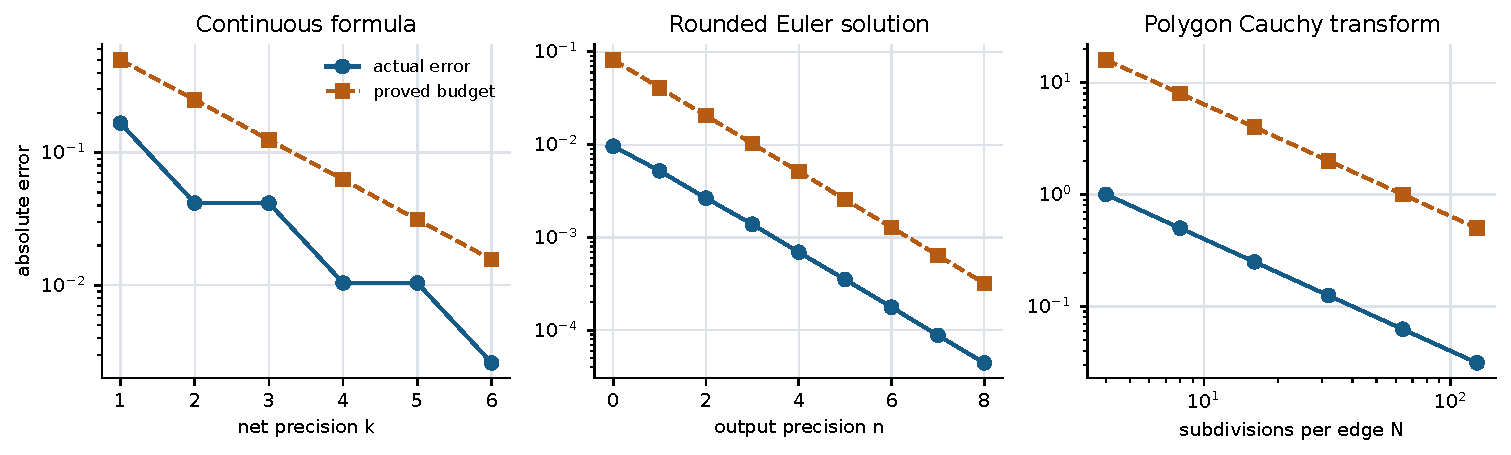
\includegraphics[width=\linewidth]{figures/validation.pdf}
\caption{Exact-rational examples, plotted after converting their final values
to floating point. Bounds are deliberately conservative. The finite checks
support implementation consistency; the universal arguments are in the text.}
\end{figure}

Run \texttt{python3 code/validate.py} from the extracted archive to reproduce
the exact checks, and \texttt{python3 code/plot\_validation.py} to regenerate
the figure. Run \texttt{pdflatex} twice on
\texttt{continuous\_mathematics\_in\_ipra.tex} to rebuild the report. The
validation receipt records that Lean compilation was not run. The source
manifest fixes the upstream commit and identifies the reviewed interfaces;
the archive does not silently substitute a newer repository state.
